\documentclass{article}
%\copyrightyear{2008}
%\pubyear{2008}

\usepackage{url}
\usepackage[numbers]{natbib}
\usepackage{graphicx}
\usepackage{multirow}

\usepackage{color}
\usepackage{xcolor}
\usepackage{listings}
\usepackage{xspace}
%\usepackage{adjustbox}
\usepackage{relsize}
\usepackage{rotating}
\usepackage{pdflscape}
\usepackage{url}
\newcommand{\prog}{{\sc Ngsane}}
\newcommand{\inlinecode}{\texttt}

\sloppy
%\linespread{1.5}

\usepackage{caption}
\DeclareCaptionFont{white}{\color{white}}
\DeclareCaptionFormat{listing}{\colorbox{gray}{\parbox{\textwidth}{#1#2#3}}}
\captionsetup[lstlisting]{format=listing,labelfont=white,textfont=white}
\lstset{language=sh,captionpos=t,tabsize=3,frame=lines,keywordstyle=\color{blue},commentstyle=\color{darkgreen},stringstyle=\color{red},numbers=left,numberstyle=\tiny,numbersep=5pt,breaklines=true,showstringspaces=false,basicstyle=\footnotesize,emph={label}}

\usepackage[margin=0.75in]{geometry}

\renewcommand\footnotemark{} % removes mark in front of footmark
\renewcommand{\bibnumfmt}[1]{{#1}. } % change numbering format in reference list
\newcommand{\natcite}[1]{\nolinebreak\citep{#1}} % nature cite to prevent superscript to appear on the next line
\newcommand{\BIBand}{\&}

\begin{document}
%\firstpage{1}
\pagestyle{empty}

\setcounter{section}{1}

\section*{Supplementary material}

\prog\ is a framework for advanced production informatics of Next Generation Sequencing libraries. Fig.~\ref{overview} visualises \prog 's functionality and structure and Tab.~\ref{Similartools} contains a list of software with similar functionality as \prog. The following sections showcase the three steps to run \prog.


\begin{figure}[ht!]
\centering
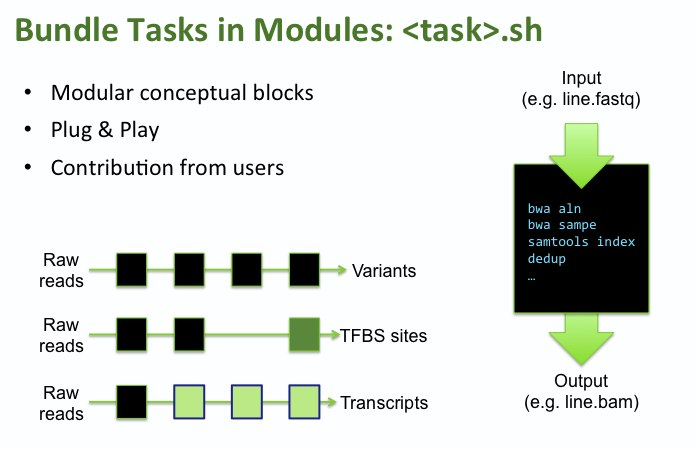
\includegraphics[width=120mm]{../../images/overview.jpg}
\caption{
{\bf Overview over \prog 's functionality and structure}. Each project (Input) has a project specific config file {\bf (A)} holding the necessary customisations for the planned analysis tasks. Note, each project can have multiple config files for each analysis task. Distinct from the project is the  \prog\ core, which contains the pan-project configuration file called {\texttt header.sh} {\bf (B)}. This file contains general system variables, platform-specific parameters, and paths to the various software binaries installed on a system. It should be configured once upon initial installation and updated as needed, for example when new software versions are installed. Also in the core is the  {\texttt trigger.sh} script {\bf (C)}, which is the main executable in \prog. 
It processes the variables and tasks specified in the configuration files, ensuring that all dependencies are met and invoking the core job submission protocols. In addition, it enables the user to selectively launch a test or 'dry' run, a full high performance computing run, or generate a summary report once the tasks have completed. {\bf (D)} The mod files contain the generic analytic pipelines that are to be executed on the HPC cluster. Each mod corresponds to a specific analysis, a single task, or a series thereof. They include checkpoints to recover previous failed executions, as well as comprehensive logging of each step. Advanced users can create customised mods and include them in the framework. After execution, a concise summary of the results and a project card {\bf(E)} can be generated. This usually includes general statistics of the results, including graphs, potential errors, and an itemised log of the checkpoints for each task.}
\label{overview}
\end{figure}

\subsection{Setup environment using toy data}
\begin{enumerate}
\item  create fastq/Run directory
\begin{small}\begin{verbatim}
-bash-4.1$ mkdir -p fastq/Run
\end{verbatim}\end{small}
\item  copy toy data to the fastq directory
\begin{small}\begin{verbatim}
-bash-4.1$ wget http://www.hpsc.csiro.au/users/bau04c/datahome/Sandbox/NGSANEDEMO/fastq/Run/RNA3kChr16.tar.gz
\end{verbatim}\end{small}
\item uncompress toy example (untar)
\begin{small}\begin{verbatim}
-bash-4.1$ tar -xvzf RNA3kChr16.tar.gz
\end{verbatim}\end{small}
\item move fastq files to fastq/Run directory 
\begin{small}\begin{verbatim}
-bash-4.1$ mv RNA3kChr16* fastq/Run
\end{verbatim}\end{small}
\item list the content of the fastq folder; it should contain one read pair but the user can deposit multiple libraries
\begin{small}\begin{verbatim}
-bash-4.1$ ls fastq/Run
RNA3kChr16_read1.fastq  RNA3kChr16_read2.fastq
\end{verbatim}\end{small}
\item copy the configuration file for \prog
\begin{small}\begin{verbatim}
-bash-4.1$ wget http://www.hpsc.csiro.au/users/bau04c/datahome/Sandbox/NGSANEDEMO/config.txt .
\end{verbatim}\end{small}
\item display the configuration file; it is currently  set up to perform mapping with Bowtie2~\citep{Langmead2012} (set RUNMAPPINGBWA="1" activates mapping with BWA~\citep{Li2009})
\begin{small}\begin{verbatim}
-bash-4.1$ cat config.txt
# author: Denis C. Bauer
# date: April 2013

#********************
# Tasks
#********************
RUNMAPPINGBOWTIE2="1" # mapping with bowtie2 set to 1 to run
RUNMAPPINGBWA="" # mapping with bwa

#********************
# Paths
#********************
SOURCE=$(pwd)
declare -a DIR; DIR=( Run )
OUT=$SOURCE
QOUT=$OUT/qout

READONE="_read1"
READTWO="_read2"
FASTQ=fastq
EXPID="Library"
LIBRARY="Provider"
PLATFORM="Illumina"

FASTA=$NGSANE_REFERENCE/b37/human_g1k_v37.fasta # needs to be set to appropriate path

\end{verbatim}\end{small}
\end{enumerate}

\subsection{Run \prog\ on toy data}
\begin{enumerate}
\item test configuration (dry run)
\begin{small}\begin{verbatim}
-bash-4.1$ trigger.sh config.txt
[NGSANE] Trigger mode: [empty] (dry run)
[NOTE] Folders: Run
[Task] bowtie2
[NOTE] setup environment
[TODO] Run/RNA3kChr16_read1.fastq
[NOTE] proceeding with job scheduling...
[NOTE] Run/RNA3kChr16
[NOTE] make Run/bowtie2/RNA3kChr16.asd.bam.dummy
[ JOB]  /apps/gi/ngsane/0.2.0//mods/bowtie2.sh 
-k /datastore/cci/bau04c/Documents/datahome/Sandbox/NGSANEDEMO/config.txt 
-f /datastore/cci/bau04c/Documents/datahome/Sandbox/NGSANEDEMO/fastq/Run/RNA3kChr16_read1.fastq 
-o /datastore/cci/bau04c/Documents/datahome/Sandbox/NGSANEDEMO/Run/bowtie2 --rgsi Run
\end{verbatim}\end{small}
\item submit a bowtie job to the cluster (Jobnumber 2187179)
\begin{small}\begin{verbatim}
-bash-4.1$ trigger.sh config.txt armed
[NGSANE] Trigger mode: armed
Double check! Then type safetyoff and hit enter to launch the job: safetyoff
... take cover!
[NOTE] Folders: Run
[Task] bowtie2
[NOTE] setup enviroment
[TODO] Run/RNA3kChr16_read1.fastq
[NOTE] proceeding with job scheduling...
[NOTE] Run/RNA3kChr16
[NOTE] make Run/bowtie2/RNA3kChr16.asd.bam.dummy
[ JOB]  /apps/gi/ngsane/0.2.0//mods/bowtie2.sh 
-k /datastore/cci/bau04c/Documents/datahome/Sandbox/NGSANEDEMO/config.txt 
-f /datastore/cci/bau04c/Documents/datahome/Sandbox/NGSANEDEMO/fastq/Run/RNA3kChr16_read1.fastq 
-o /datastore/cci/bau04c/Documents/datahome/Sandbox/NGSANEDEMO/Run/bowtie2 --rgsi Run
Jobnumber 2187179
\end{verbatim}\end{small}
\end{enumerate}

\subsection{Aggregate results in a summary report}
To have a one page overview of job success, and results we now generate the Project Card
\begin{small}\begin{verbatim}
-bash-4.1$ trigger.sh config.txt report
[NGSANE] Trigger mode: report
>>>>> Generate HTML report
>>>>> startdate Mon Sep 23 17:02:31 EST 2013
>>>>> hostname burnet-login
>>>>> makeSummary.sh -k /datastore/cci/bau04c/Documents/datahome/Sandbox/NGSANEDEMO/config.txt
--R           --
 R version 3.0.0 (2013-04-03) -- "Masked Marvel" Copyright (C) 2013 The R Foundation for Statistical Computing 
 Platform: x86_64-unknown-linux-gnu (64-bit)
--Python      --
 Python 2.7.2
QC - bowtie2
>>>>> Generate HTML report - FINISHED
>>>>> enddate Mon Sep 23 17:02:33 EST 2013
\end{verbatim}\end{small}

\begin{figure*}[h!]
    \centering
   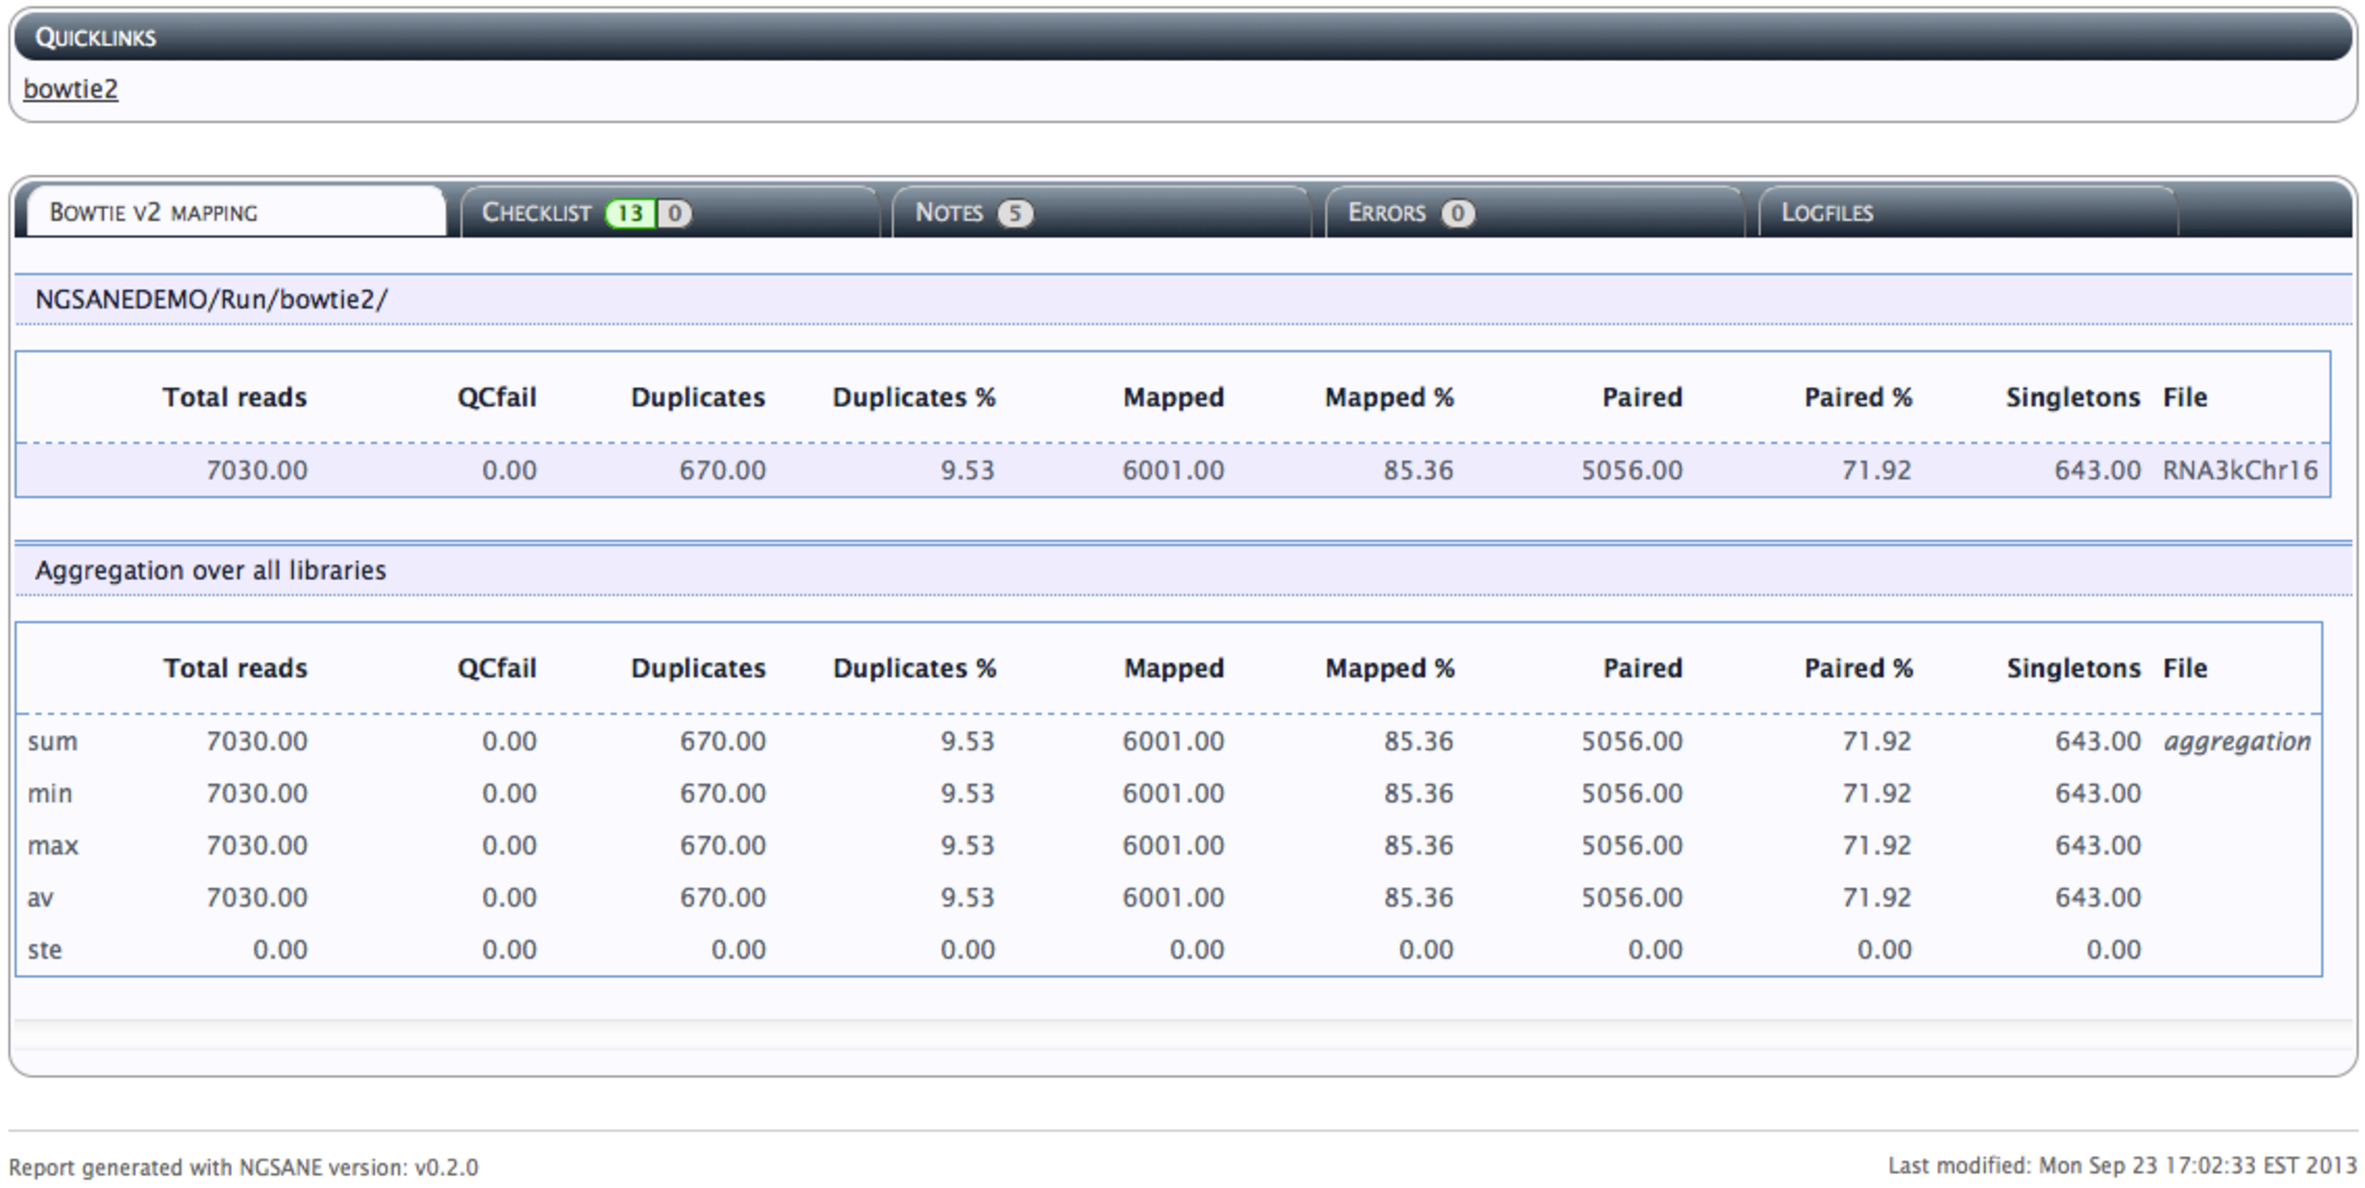
\includegraphics[type=pdf,ext=.pdf,read=.pdf, scale=0.4]{NGSANEprojectcard}
    \caption{
      {\bf Example project card}} 
      \label{fig:overview}
\end{figure*}

The Project Card (Fig. \ref{fig:overview}) can be created at the very end of the execution or at any intermittent step allowing human quality control throughout the stages of a project. The "Notes" and "Error" tabs specifically highlight, which (if any) subset of files contain error and the "Logfile" tab facilitates easy access to the specific log files to identify the source of the problem. Once the faulty files are identified and the error is removed \prog\ allows the automated resubmission of the file-subset starting from the point of error. 

More comprehensive reports that include summary graphics area available from:

\url{http://www.hpsc.csiro.au/users/bau04c/datahome/Sandbox/smokebox_ngsane/smokebox/result/}

\newpage

\begin{landscape}

\begin{table}[htdp]
\tiny 
\caption{Available academic or commercial software for NGS data analysis}
\begin{center}
\begin{tabular}{|p{2cm}|p{0.6cm}|p{1cm}|p{2cm}|p{1cm}|p{1cm}|p{1cm}|p{1cm}|p{1cm}|p{1cm}|p{1cm}|p{1cm}|p{4cm}|}
\hline
Name & Date & comercial & Domain specific & language & subset files & recovery & pipelining & paralleli-zation & hpc & hadoop & automatic summary & URL \\
\hline
NGSANE & 2013 & academic & no & BASH & yes & yes & yes & yes & yes & not yet & yes & \url{https://github.com/BauerLab/ngsane} \\
Nestly~\cite{McCoy2013} & 2013 & academic & no & python & yes & no & no & no & no & no & yes & \url{http://github.com/fhcrc/nestly} \\
RUbioSeq~\cite{Rubio-Camarillo2013} & 2013 & academic & bisulfite and exome variants & perl &  &  & yes & yes & SGE & no & no & \url{http://rubioseq.sourceforge.net/.} \\
Bpipe~\cite{Sadedin2012} & 2012 & academic & no & Groovy &  & yes & yes & yes & yes & no & yes & \url{http://bpipe.org} \\
GeneProf~\cite{Halbritter2012} & 2012 & academic & no & Webserver &  &  &  &  &  &  &  & \url{http://www.geneprof.org/GeneProf/} \\
GenomicTools~\cite{Tsirigos2012} & 2012 & academic & no & C++ & yes & no & yes & yes & no & no & no & \url{http://code.google.com/p/ibm-cbc-genomic-tools} \\
PGAP~\cite{Zhao2012} & 2012 & academic & pan-genomic analysis & Perl &  &  &  &  &  &  &  & \url{http://pgap.sourceforge.net/} \\
Snakemake~\cite{Koester2012} & 2012 & academic & no & python & yes &  & yes &  & not yet &  &  & \url{https://code.google.com/p/snakemake/} \\
NARWHAL~\cite{Brouwer2012} & 2012 & academic & de-multiplexing & python, BASH, c &  &  & yes & yes & no & no & yes & \url{https://trac.nbic.nl/narwhal/} \\
SeqWare~\cite{OConnor2010} & 2010 & academic &   &  HBase based & yes  & yes  & yes & yes & yes & yes &  yes & \url{http://seqware.github.io} \\
CLoVR~\cite{Angiuoli2011} & 2011 & academic & yes & Webserver &  &  &  & yes & no & yes &  & \url{http://clovr.org/} \\
Conveyor~\cite{Linke2011} & 2011 & academic & no & .NET &  &  &  & yes & no &  &  & \url{http://conveyor.cebitec.uni-bielefeld.de} \\
Knime4Bio~\cite{Lindenbaum2011} & 2011 & academic & yes & Webserver &  &  &  &  &  &  &  & \url{http://code.google.com/p/knime4bio/} \\
PaPy~\cite{Cieslik2011} & 2011 & academic & no & python &  &  & yes & yes &  &  &  & \url{http://muralab.org/PaPy/} \\
Pyicos~\cite{Althammer2011} & 2011 & academic & no & python &  &  &  &  &  &  &  & \url{http://regulatorygenomics.upf.edu/pyicos} \\
NGS\_backbone~\cite{Blanca2011} & 2011 & academic & no &  &  &  & yes & yes &  &  &  & \url{http://bioinf.comav.upv.es/ngs\_backbone/} \\
Galaxy~\cite{Goecks2010} & 2010 & academic & no & Webserver & yes & yes & yes & no & no &  & no &  \\
Ruffus~\cite{Goodstadt2010} & 2010 & academic & no & python & yes & yes &  &  &  &  &  & \url{http://www.ruffus.org.uk/} \\
CrossBow~\cite{Langmead2009} & 2009 & academic & SNP calling & C++ &  &  &  &  &  & yes &  & \url{http://bowtie-bio.sourceforge.net/crossbow/index.shtml} \\
Mobyle~\cite{Neron2009} & 2009 & academic & no & Webserver & yes &  & no &  &  &  &  &  \\
Ipython~\cite{Perez2007} & 2007 & academic & no & python & yes & yes & yes & yes & yes &  & no & \url{http://ipython.org/} \\
Taverna~\cite{Oinn2004} & 2004 & academic & no & Webserver & yes & yes & yes & no & no &  &  & \url{http://www.taverna.org.uk/} \\
Biopipe~\cite{Hoon2003} & 2003 & academic & no & Webserver &  &  &  &  &  &  &  &  \\
GATK Queue &  & academic & GATK commands & JAVA &  &  &  &  &  &  &  & \url{http://gatkforums.broadinstitute.org/discussion/1306/overview-of-queue} \\
Gene Pattern &  & academic &  & Webserver &  &  &  &  &  &  &  & \url{http://www.broadinstitute.org/cancer/software/genepattern} \\
ISGA &  & academic & prokaryotic annotation and prokaryotic assembly & Webserver &  &  &  &  &  &  &  & \url{http://gmod.org/wiki/ISGA} \\
Kepler &  & academic &  & Webserver & yes &  & no &  & yes &  &  &  \\
Pegasus &  & academic &  & Webserver & yes &  &  &  & yes &  &  &  \\
GeneSpring &  & Agilent &  &  &  &  &  &  &  &  &  & \url{http://www.genomics.agilent.com} \\
Avadis NGS &  & Avadis NGS &  &  &  &  &  &  &  &  &  & \url{http://www.avadis-ngs.com/} \\
Genomics Workbench &  & CLC Bio &  &  &  &  &  &  &  &  &  & \url{http://www.clcbio.com/} \\
DNASTAR &  & DNASTAR &  &  &  &  &  &  &  &  &  & \url{http://www.dnastar.com} \\
CASAVA &  & illumina &  &  &  &  &  &  &  &  &  & \url{http://www.illumina.com/software/genome\_analyzer\_software.ilmn} \\
NextGENe &  & NextGENe &  &  &  &  &  &  &  &  &  & \url{http://www.softgenetics.com/NextGENe.html} \\
Partek &  & Partek &  &  &  &  &  &  &  &  &  & \url{http://www.partek.com/?q=ngs} \\
geospiza &  & Perkin-Elmer &  &  &  &  &  &  &  &  &  & \url{http://www.geospiza.com/ & } \\
\hline
\end{tabular}
\end{center}
\label{Similartools}
\caption{{\bf Software similar to \prog .} Tools are listed in no particular order and the list may not be comprehensive. See https://github.com/BauerLab/ngsane/wiki/Similar-Projects for an up-to-date list.}
\end{table}%

\end{landscape}

\bibliographystyle{natbib}
\bibliography{ngsane}

\end{document}




